\documentclass[letterpaper,twocolumn,amsmath,amssymb,floatfix,aps,superscriptaddress]{revtex4}
\usepackage{geometry}                % See geometry.pdf to learn the layout options. There are lots.
\geometry{letterpaper}                   % ... or a4paper or a5paper or ... 
%\geometry{landscape}                % Activate for for rotated page geometry
%\usepackage[parfill]{parskip}    % Activate to begin paragraphs with an empty line rather than an indent
\usepackage{graphicx}
\usepackage{epstopdf}
\usepackage{hyperref}
%\usepackage{jheppub}
\usepackage{color}
%\usepackage{pstricks}
\usepackage{bm}  % bold math
\usepackage{epsfig}


\def\ul#1#2{\textstyle{\frac{#1}{#2}}}
\def\tr{{\mathrm{Tr}}}
\newcommand {\vct}[1] {\mathbf {#1}}

\renewcommand{\labelenumi}{(\roman{enumi})}

\begin{document}

\title{Dielectric response variation and the strength of van der Waals interactions}

\author{Jaime E. Hopkins}\email{hopkins@physics.umass.edu}
\affiliation{Department of Physics, University of Massachusetts, Amherst, MA 01003, USA}

\author{Daniel M. Dryden} 
\affiliation{Department of Materials Science and Engineering, Case School of Engi- neering, Case Western Reserve University, Cleveland Ohio, 44106-7204,}

\author{Wai - Yim Ching} 
\affiliation{Department of Physics and Astronomy, University of Missouri-Kansas City, Kansas City, Missouri 64110}

\author{Roger H. French}
\affiliation{Department of Materials Science and Engineering, Case School of Engineering, Case Western Reserve University, Cleveland Ohio, 44106-7204,}

\author{V. Adrian Parsegian}
\affiliation{Department of Physics, University of Massachusetts, Amherst, MA 01003, USA}

\author{Rudolf Podgornik}
\affiliation{Department of Physics, University of Massachusetts, Amherst, MA 01003, USA}
\affiliation{Department of Theoretical Physics, Jo\v{z}ef Stefan Institute, SI-1000 Ljubljana, Slovenia}
\affiliation{Department of Physics, Faculty of Mathematics and Physics, University of Ljubljana, SI-1000 Ljubljana, Slovenia}


\begin{abstract}
~
\end{abstract}

\maketitle

The general theory of long range (macro)molecular van der Waals (vdW) forces is well established \cite{Parsegian,Bordag}, but there are  nevertheless important issues that are widely misunderstood and deeply entrenched in the colloid and nano-science community. While it is clear that in the Lifshitz theory of vdW forces, the interaction free energy is a {\sl functional} of the dielectric response function at imaginary Matsubara frequencies (itself a functional of the imaginary part of the total dielectric response function via the Kramers-Kronig relations), it remains seldom appreciated exactly how this non-locality in the dielectric response acts in the properties of vdW interaction. What is also often misunderstood is what are the actual quantitative consequences of variations in the dielectric response of the interacting media on the magnitude of vdW interactions. 

There are two important contexts in which the appreciation of such issues is a {\sl sine qua non} for the
understanding of the overall features of the interaction between colloidal or nano particles. In the first case, {\sl refractive index matching}, changes in the dielectric response functions of the medium between the interacting dielectrics is used to modify the inter particle interactions through their vdW component . For a relatively recent selection of papers see \cite{Blaaderen,Chaikin,Bonn,Shen,Manohar}.  Here one often assumes that the dielectric response is dominated by a single adsorption peak in the optical frequency regime, corresponding to electronic properties of the materials. The strength of the vdW interaction, as codified by the Hamaker coefficient \cite{Parsegian}, then appears as a simple function of the difference between the squares of the refractive index of the medium and the interacting bodies \cite{Isrealachvili}. If the zero frequency dielectric response is small, matching the refractive index at this single adsorption peak should effectively quench the long range vdW component of molecular interactions. While a tempting simplification, this could lead to gross underestimation of the overall strength of (macro)molecular interactions, possibly precluding correct interpretation of experimental data on {\sl e.g.} wetting.

Another important context for the intricacies of the effect non-locality in the dielectric response  on the variation of the vdW interaction, one into which we shall delve more deeply, is the effect of {\sl excitonic peaks} in the optical regime of, {\sl e.g.},  single-walled carbon nanotubes (SWCNTs) \cite{CNTexciton}. Excitons introduce additional peaks in  the energy range below 5 eV or slightly shift the position of some other peaks in SWCNTs. They are measurable \cite{Measurable} and are, of course, very important  for optical properties of these materials. Their importance for the strength of vdW interaction in the context of SWCNTs remains less clear. Recently Hobbie and co-workers \cite{Hobbie} used a simple empirical approach to assess the effect of the excitonic peaks on the strength of vdW interactions between SWCNTs. They concluded that in the case of semiconducting nanotubes, neglecting the three excitonic resonances in the optical regime reduces the Hamaker coefficient by roughly 5 \%. For metallic SWCNTs, neglect of either of these terms reduces the Hamaker coefficient by roughly 3\%. In this view, excitonic effects should have a qualitatively small but nevertheless measurable effect, but its exact magnitude has to be evaluated by more detailed calculations. It appears that the importance of a certain spectroscopic feature in, {\sl e.g.}, the optical regime does not necessarily translate directly into an equally important feature of vdW interactions. What {\sl exactly} is the connection remains unclear.

The same problem of excitonic peaks and their influence on the overall strength of vdW interaction appears also between condensed media. In this case the theoretical method of choice to evaluate the electronic properties is the orthogonalized linear combination of atomic orbital (OLCAO) variant of density functional theory (DFT), which uses local atomic orbitals for the basis expansion rather than the plane waves \cite{DFT}.  This methodology formulated on a one-electron level of course precludes the inclusion of many-body excitonic corrections, as they are not compatible with the OLCAO-DFT context. Since excitonic effects due to the many-body interactions are therefore not considered on this level, there may be concerns about the underestimation of the band gap as well as a possible rescaling of the complete spectrum. This necessarily implies also modifications in the overall magnitude of the vdW interactions between the condensed media. As an example of OLCAO-DFT type of calculation, one can consider the dielectric permittivity of amorphous silica \cite{silica} that can be compared with direct experiments \cite{Tan}. This comparison shows that the one-electron level OLCAO-DFT calculations can not reproduce the measured excitonic peak. Again the question remains as to how relevant is this omission in the overall features of the optical response for the quantitative evaluation of the corresponding strength of the vdW interaction.

In order to address all these queries, we will investigate in detail the effect of variation in the spectral properties of the dielectric response function over a finite interval of frequencies on the strength of the vdW interactions as quantified by the Hamaker coefficient. We will confine ourselves to the non-retarded regime as well as to planar interaction geometry, but the analysis can be straightforwardly repeated also for, {\sl e.g.}, small spherical particles or in fact for any geometry for which there are explicit Lifshitz results \cite{Parsegian}. We will first analyse a simple toy model for the variation of the dielectric response function and then apply the general theory to an actual dielectric response spectrum with/without the excitonic peak and assess the variation wrought by changes in the dielectric spectrum on the corresponding Hamaker coefficient.

%\begin{figure}[h]
%\centerline{\includegraphics[width=8cm]{./Untitled.pdf}}
%\caption{Figure 1.\label{fig1}}
%\end{figure}

%\subsection{Non-retarded case}

\subsection{Interaction free energy variation: general}

Assume that the spectral response of two interacting planar dielectric surfaces is changed from  $ \varepsilon(\omega) \longrightarrow \varepsilon(\omega) + \delta \varepsilon(\omega) $. The Kramers-Kronig transform that enters the vdW interaction free energy is in general defined as 
\begin{equation}
\varepsilon(i \zeta) = 1 + \frac{2}{\pi} \int_0^{\infty} \frac{\omega ~{\varepsilon'' (\omega)}}{\omega^2 + \zeta^2}d\omega,
\label{cgsrlhjk}
\end{equation}
with $\varepsilon'' (\omega)$ the imaginary part of $ \varepsilon(\omega)$. Quite generally $\varepsilon(i \zeta)$ is a real, monotonically decreasing function of its argument $\zeta$. It follows from the Lifshitz theory \cite{LLSPpart2} that the corresponding interaction free energy change is then defined as $\delta {\cal F} = {\cal F}[\varepsilon(i \zeta) + \delta \varepsilon(i \zeta)] - {\cal F}[\varepsilon(i \zeta)]$. For the planar case of vdW interaction between two semiinfinite layers, one obtains to the lowest (linear) order in the dielectric response change $\delta \varepsilon$ the simple result \cite{LLSPpart2} 
\begin{widetext}
\begin{equation}
\delta {\cal F} = - \frac{k_BT}{4\pi} {\sum_{N=0}^{\infty}}'  \zeta_N^2\!\!\left( {\rm Tr} \int_{(V)} \!\!\!\!\!\!{\cal D}_{ik}(i \zeta_N, {\bf r}, {\bf r}) d^3{\bf r} \right) \delta \varepsilon(i \zeta_N) = - \frac{k_BT}{4\pi} S  {\sum_{N=0}^{\infty}}'  \zeta_N^2\!\!\left( {\rm Tr} \int_{(z)} \!\!\!\!\!\!{\cal D}_{ik}(i \zeta_N, z, z) d{z} \right) \delta \varepsilon(i \zeta_N).
\label{cnshirugl}
\end{equation}
\end{widetext}
The last identity in the above equation stems from the presumed planar geometry with  surface area  $S$ of the interacting interfaces.  The sum is over the Matsubara frequencies, $\zeta_N = 2\pi N k_BT/\hbar$, where $N$ is an integer and the $N=0$ term is counted with a weight $1/2$. At room temperature the Matsubara frequencies are a multiple of $\rm 2.4 \times 10^{14}~s^{-1}$ and thus cover the whole frequency regime rather unevenly. While only a single $\zeta_N$, i.e. $\zeta_0$,  corresponds to the static response, several for the IR frequencies and a whole band of Matsubara frequencies fall within the optical and UV regimes, it is inadmissible to conclude from this that the optical and UV regimes therefore typically dominate the properties of the vdW interaction. This interaction is a functional of $\varepsilon(i \zeta_N)$ and not $\varepsilon(\zeta_N)$, the connection being provided by the non-local London-vdW transform, Eq. \ref{cgsrlhjk}. Because of this non-locality variation in the spectral properties of the interacting media at a certain frequency is not directly related to the corresponding frequency term variation in the Matsubara summation of the vdW interaction free energy.

% except in the case of vdW interactions mediated by water, where the infrared and microwave components of the dielectric spectrum of water make the $N=0$ term dominant even at relatively large separations \cite{NinPar-water}.

Limiting ourselves to the case of planar parallel interfaces between two semi-infinite media separated by distance $D$ with dielectric response function $\epsilon(\omega)$ and an intervening medium of $\epsilon_m(\omega)$, the vdW interaction free energy per unit surface area in the non-retarded limit is given by \footnote{Parsegian} 
$${{\cal F}(D)}/{S} =  - \frac{{\cal H}}{(12\pi D^2)} %\qquad {\rm so~that} \qquad \delta \bigg(\frac{{\cal F}(D)}{S}\bigg) =  - \frac{\delta {\cal H}}{12\pi D^2}.
\label{cfbr}$$ where ${\cal H}$, the {\em Hamaker coefficient}, is defined as
\begin{equation}
{\cal H} = \frac32 k_BT {\sum_{N=0}^{\infty}}'\!\! \int_0^{\infty} \!\!\! \!\!\! u \log\bigg( 1 - \overline\Delta_{12}^2(i \zeta_N) e^{-u}\bigg) du\,,
\label{vdxahj}
\end{equation}
with the dielectric contrast given by
\begin{eqnarray}
 \overline\Delta_{12}(i \zeta_N) &=& \left( \frac{\epsilon(i \zeta_N) - \epsilon_m(i \zeta_N)}{\epsilon(i \zeta_N) + \epsilon_m(i \zeta_N)}\right). \nonumber\\
~
\end{eqnarray}
$\epsilon(i \zeta_N)$ is the London-vdW dispersion transform Eq. \ref{cgsrlhjk} of the dielectric responses of the two semiinfinite slabs and $\epsilon_m(i \zeta_N)$ is the same for the medium in between, both evaluated at Matsubara frequencies. It then follows quite straightforwardly that the interaction free energy for the vdW interaction of two semi-infinite slabs is  
\begin{eqnarray}
\kern-10pt \frac{{\cal F}(D)}{S} &=&  - \frac{k_BT }{8\pi D^2} {\sum_{N=0}^{\infty}}'  Li_3(\overline\Delta_{12}^2(i \zeta_N) ),
%\nonumber\\
%&=& - \frac{k_BT }{8\pi D^2} {\sum_{N=0}^{\infty}}'  \sum_{M=1}^{\infty} \frac{(\overline\Delta_{12}^2(i \zeta_N))^M}{M^3}.
\label{cfbr1}
\end{eqnarray}
where the polylog function $\text{Li}_{\nu}(z)$ is defined in a standard way \cite{Abramowitz}. The variation of this interaction free energy corresponding to a small variation in the dielectric response functions of the interacting bodies can then be obtained as
\begin{widetext}
\begin{equation}
\kern-5pt \delta \bigg(\frac{{\cal F}(D)}{S}\bigg) = - \frac{k_BT}{8\pi ~D^2} ~{\sum_{N=0}^{\infty}}'  {\text{Li}_2\left(\overline\Delta_{12}(i \zeta_N) ^2\right)}~ \frac{\bigg( 1 - \overline\Delta_{12}(i \zeta_N)^2 \bigg)}{\overline\Delta_{12}(i \zeta_N)}  \frac{\delta \epsilon(i \zeta_N)}{\epsilon(i \zeta_N)} = - \frac{k_BT}{8\pi ~D^2} ~{\sum_{N=0}^{\infty}}'  \delta{\cal A}(i\zeta_N).
\label{ncirselunh}
\end{equation}
\end{widetext}
This free energy variation could be derived also from the general result, Eq. \ref{cnshirugl},  for the specific case of  planar semi-infinite interaction geometry in the non-retarded limit. We next investigate  the dependence of the terms in the above Matsubara sum on the value of the frequency.  While the relative change in the dielectric response function ${\delta \epsilon(i \zeta)}/{\epsilon(i \zeta)}$ is a monotonic function, the factor multiplying it in  Eq. \ref{ncirselunh}, $ {\text{Li}_2\left(\overline\Delta_{12}(i \zeta) ^2\right)}~ {\left( 1 - \overline\Delta_{12}(i \zeta)^2 \right)}/{\overline\Delta_{12}(i \zeta)},$ is not.  As a consequence, the contribution of the various terms, $\delta{\cal A}(i\zeta_N)$,  to the total Matsubara sum has a maximum whose position depends on the exact form of $\delta \epsilon(i \zeta)$ and $\epsilon(i \zeta)$. This can make the connection between the variation in the dielectric spectrum and the corresponding variation in the vdW interaction free energy quite complicated.


\subsection{Interaction free energy variation: toy model}

In order to analyze the dependence $\delta{\cal A}(i\zeta)$, we need a form for the frequency dependence of the dielectric function. For this we introduce a simplified "toy" model that will reveal the salient features of the more realistic problem addressed later. 

We assume a dielectric response with its imaginary part equal to  $ {\varepsilon'' (\omega)} = {\varepsilon''_0 (\omega)}  \label{dhds}$. This dielectric response we then modify by addition of a single narrow absorption peak centered at the frequency $\omega_0$ with a line width ${A}$ approximated as ${\delta\varepsilon'' (\omega)} = A~ \delta(\omega - \omega_0)$. $A$ is obviously proportional to the full width at half maximum as $\rm FWHM \simeq 2 \sqrt{2 \log{2}} A$.
%\begin{equation}
%\int_{\omega_0} d\omega~ {\varepsilon'' (\omega)} = {\cal A},
%\label{dhds1}
%\end{equation}
This defines our toy model. Later we will upgrade it to a realistic calculation for amorphous silica with and without the excitonic peak.

From these model assumptions, we then obtain the relevant Kramers-Kronig transforms as 
\begin{equation}
\label{nslrvgnv}
\varepsilon(i \zeta) = 1 + \frac{2}{\pi} \int_0^{\infty} \frac{\omega ~{\varepsilon_0'' (\omega)}}{\omega^2 + \zeta^2}d\omega = 1 + \varepsilon_0 (i \zeta) 
\end{equation}
and
\begin{equation} 
\delta \varepsilon(i \zeta) = \frac{2}{\pi} \int_0^{\infty} \frac{\omega ~{\delta\varepsilon'' (\omega)}}{\omega^2 + \zeta^2}d\omega = \frac{2}{\pi} \frac{\omega_0 ~{A} }{\omega_0^2 + \zeta^2}.
\label{ngkslh}
\end{equation}
Assuming furthermore for convenience that the medium is a vacuum, $\varepsilon_m \equiv 1$, we then have
\begin{equation}
 \overline\Delta_{12}(\varepsilon_0(i \zeta)) = \frac{ \varepsilon_0 (i \zeta)}{2 + \varepsilon_0 (i \zeta)}.
 \end{equation}
What we are looking for now is the change in vdW interaction free energy as the $\omega_0$ peak is added, {\sl viz}. as the dielectric response changes from $ \varepsilon(i \zeta) = 1 + \varepsilon_0 (i \zeta)$ to $\varepsilon(i \zeta) = 1 + \varepsilon_0 (i \zeta) + \delta \varepsilon(i \zeta)$. Our goal is to obtain the free energy difference on introduction of a single absorption peak at $\omega_0$.

\begin{figure*}[t!]
\begin{center}
\begin{minipage}[b]{0.41\textwidth}
\begin{center}
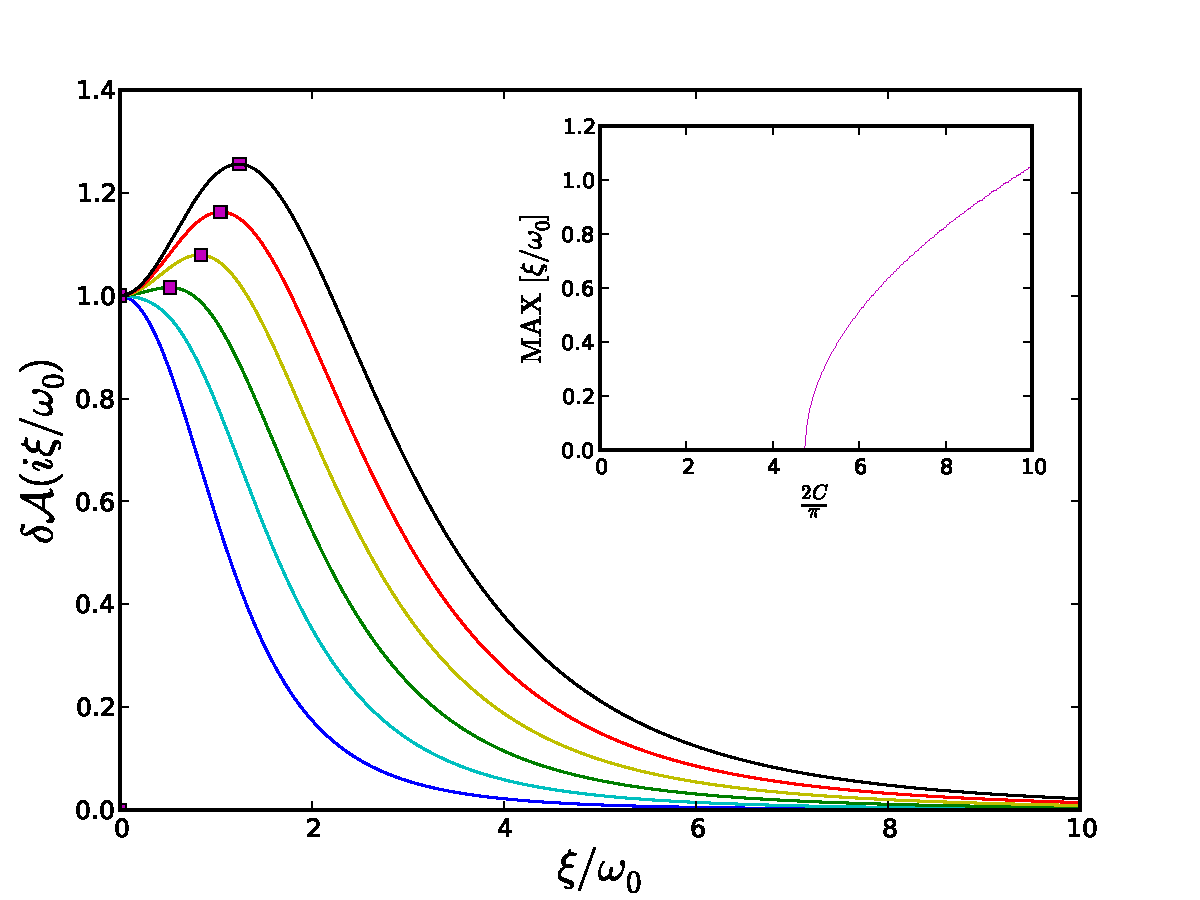
\includegraphics[width=1.2\textwidth]{./130807_plots/130812_Hopkins_updated_fig_1a.pdf} (a)
\end{center}
\end{minipage}
\hskip 43pt
\begin{minipage}[b]{0.41\textwidth}
\begin{center}
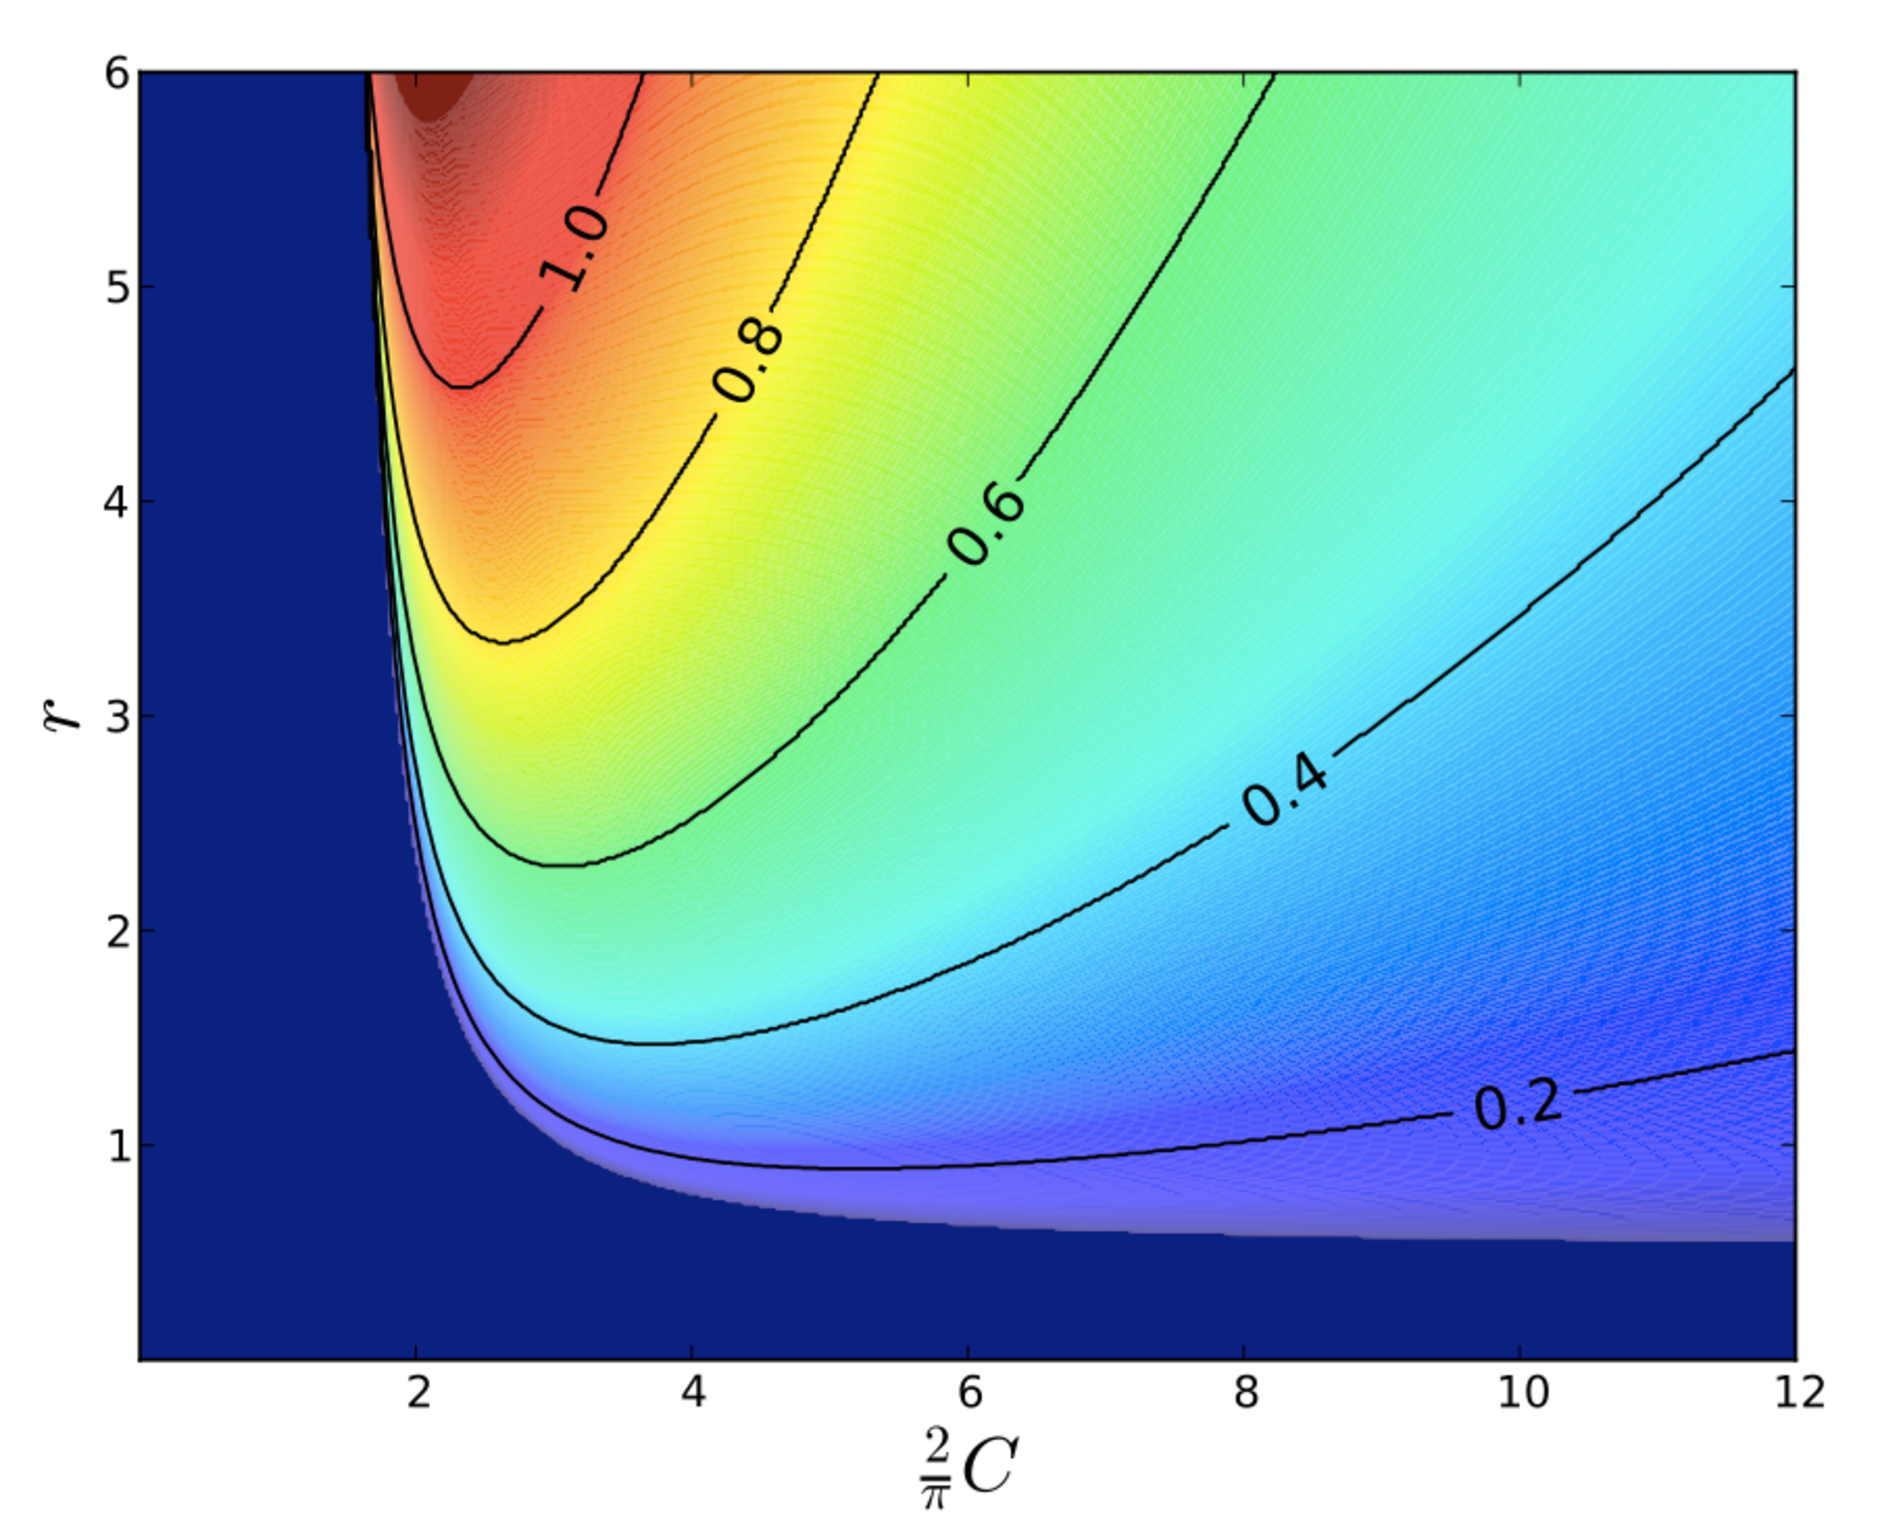
\includegraphics[width=1.06\textwidth]{./130807_plots/fig1b_contour_xi_max-dilute.pdf} (b)
\end{center}
\end{minipage}
\caption{(a) The function $\delta{\cal A}(i\zeta)$, Eq. \ref{ncirselunh}, for six different values of ${\frac{2}{\pi} {\cal C}}$ (from 2 to 12, top to bottom) as a function of $(\zeta/\omega_0)$. With increase of ${\cal C}$ the maximum (purple squares) moves from zero frequency toward non-zero values. The inset shows the complete dependence of the maximum of $\delta{\cal A}(i\zeta)$, $\zeta_{max}$, on $\cal C$. For this calculation, we took $r = \omega_0/\tilde\omega_0 = 1$. (b) Contour plot of $Max\left(\delta{\cal A}(i\zeta)\right)$ as a function of  ${\cal C}$ as well as $r = \omega_0/\tilde\omega$.}
\label{fiddle1}
\end{center}
\end{figure*} 

We proceed with some general observations. The expression for the London-vdW transform Eq. \ref{nslrvgnv} has the following two limits
for $ \zeta \longrightarrow 0$ and $\zeta \longrightarrow \infty$, respectively
\begin{equation}
\kern-5pt \varepsilon (i \zeta) \simeq \left\{
\begin{array}{cc}
1 + \frac{2}{\pi} {\int_0^{\infty}} \omega^{-1}{{\varepsilon'' (\omega)}}d\omega = 1 + \frac{2}{\pi} {\cal C} & \\
~ & ~ \\
1 + \frac{2}{\pi} \zeta^{-2} {\int_0^{\infty}} \omega ~{{\varepsilon'' (\omega)}}d\omega = 1 +  \zeta^{-2} \frac{2}{\pi}{\cal C}' &  \\
\end{array}
\right. .
\label{qcnofiwun}
\end{equation}
In the first integral we recognize the static limit sum rule and in the second one the oscillator strength sum rule (for details see Ref. \cite{Smith}). The latter relates the integral of $\omega ~{\rm Im} ~\varepsilon (\omega)$ with the effective number of electrons used in transitions at all energies. The two limits in Eq. \ref{qcnofiwun} then suggest a convenient approximation covering the whole range of frequencies that will allow us to analyze the corresponding vdW interaction free energy. It has the form 
\begin{equation}
\varepsilon_0 (i \zeta) \simeq  \frac{(\varepsilon(0) - 1)}{1 + \left(\frac{\zeta}{\omega_0}\right)^{2}\left(\frac{\omega_0}{\tilde\omega}\right)^2}, 
\label{cmjlčl}
\end{equation}
with $\tilde\omega^2  = {\cal C'}/{{\cal C}}$ where we take ${\cal C} = \frac{\pi}{2}(\varepsilon(0) - 1)$.  This approximation is, in fact, quite accurate as long as the dielectric response is given by a single band of frequencies in the optical and/or UV regimes. It becomes inadequate when there are contributions to ${\varepsilon'' (\omega)}$ also from the IR and MW regimes. In that case, one should simply revert to the exact definition Eq. \ref{nslrvgnv}. From the sum rules \cite{Smith}, it follows that $\tilde\omega$  can be written explicitly as
\begin{equation}
\tilde\omega^2 = \frac{{\int_0^{\infty} \omega ~{{\varepsilon'' (\omega)}}d\omega}}{{{\int_0^{\infty}} \omega^{-1}{{\varepsilon'' (\omega)}}d\omega}} = \frac{\omega_p^2}{(\varepsilon(0) - 1)},
\end{equation}
where $\omega_p$ is the plasma frequency depending on the number of electrons and $\varepsilon(0) $ is the static dielectric constant. We expressed the $\zeta$ dependence in terms of the dimensionless variable $(\zeta/\omega_0)$ because of the assumed form of $\delta \varepsilon(i \zeta)$, Eq. \ref{ngkslh}, that depends on this dimensionless combination. The form Eq. \ref{cmjlčl} now allows us to deduce some general aspects of the vdW interaction free energy variation. 


%\begin{figure} 
%\begin{center}
%\includegraphics[width=0.5\textwidth]{130731_Hopkins_CORRECT_y_with_ymax_inset.pdf} 
%\end{center}
%\caption{The function $\delta{\cal A}(i\zeta)$ for six different values of ${\frac{2}{\pi} {\cal C}}$ (from 2 to 12, top to bottom) as a function of $(\zeta/\omega_0)$. On increase of ${\cal C}$ the maximum moves from zero frequency towards non-zero values. The inset shows the complete dependence of the maximum of $\delta{\cal A}(i\zeta)$, $\zeta_{max}$, on $\cal C$. For this calculation we took $r = \omega_0/\tilde\omega_0 = 1$. }
%\label{fiddle1}
%\end{figure} 

%\begin{figure}[t!]
%\begin{center}
%\includegraphics[width=0.5\textwidth]{threeD.pdf} 
%\end{center}
%\caption{The dependence of $Max\left(\delta{\cal A}(i\zeta)\right)$ on ${\cal C}$ as well as $r = \omega_0/\tilde\omega$.}
%\label{3D}
%\end{figure} 


Having the explicit form of $\varepsilon_0 (i \zeta)$, we can now calculate the dependence of $\delta{\cal A}(i\zeta)$ on the ratio $\zeta/\omega_0$ (see Fig. \ref{fiddle1}). This dependence shows a maximum that depends on the values of $ {\frac{2}{\pi} {\cal C}}$ and the ratio $r = \omega_0/\tilde\omega$. Obviously as ${\cal C}$ grows past a fixed value, found numerically to be ${\cal C}_0 \simeq 7.38$ (see below), the maximum of $\delta{\cal A}(i\zeta)$ is displaced from $\zeta = 0$ to non-zero values. This means that the maximum contribution to the vdW interaction free energy is given by the zero frequency term for  ${\cal C} < {\cal C}_0$ and then depends monotonously on ${\cal C}$ for larger values. In fact, the behavior of $Max\left(\delta{\cal A}(i\zeta)\right)$ on ${\cal C}$ bears a striking formal resemblance to the temperature dependence of the order parameter close to a second order phase transition. 

\begin{figure*}[t!]
\begin{center}
\begin{minipage}[b]{0.45\textwidth}
\begin{center}
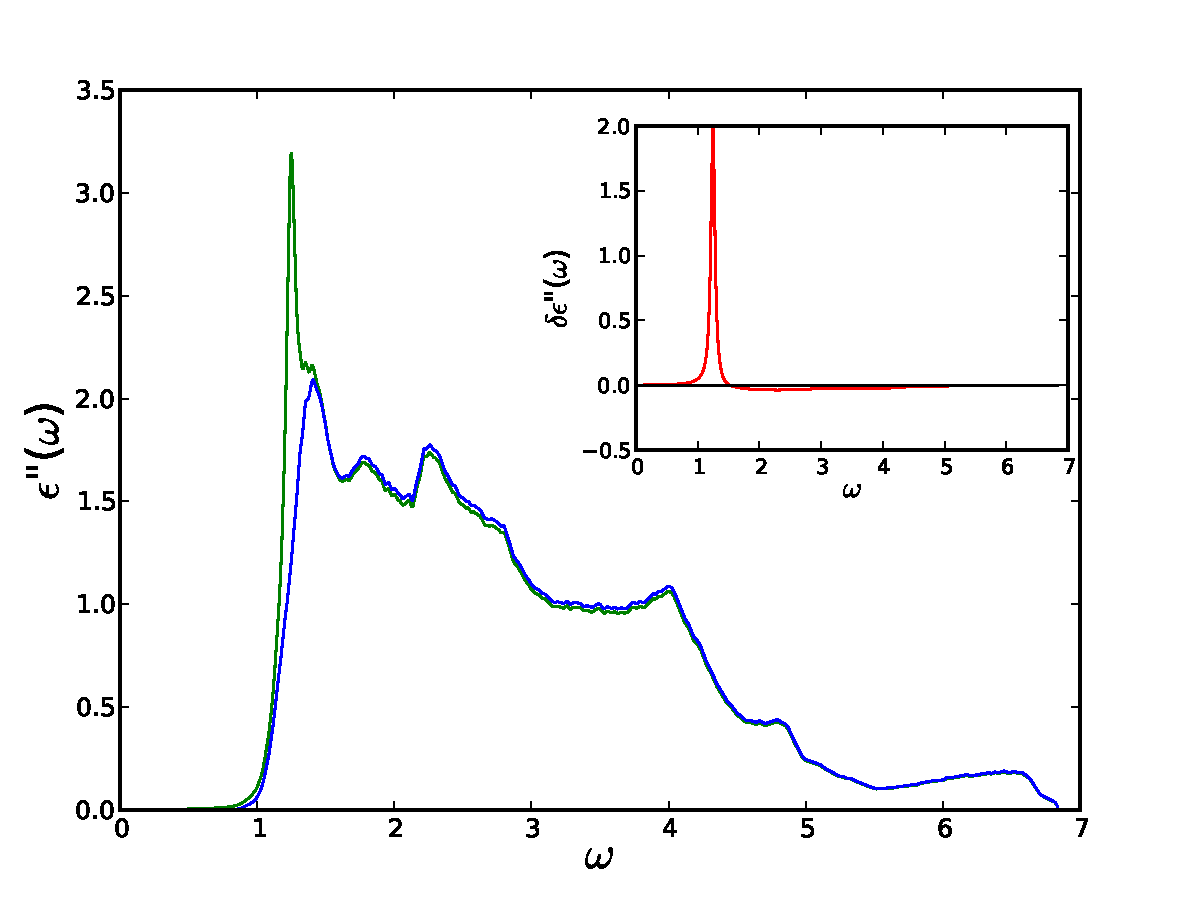
\includegraphics[width=1.2\textwidth]{./130807_plots/fig2a_eps2_deps2.pdf} (a)
\end{center}
\end{minipage}
\hskip 34pt
\begin{minipage}[b]{0.45\textwidth}
\begin{center}
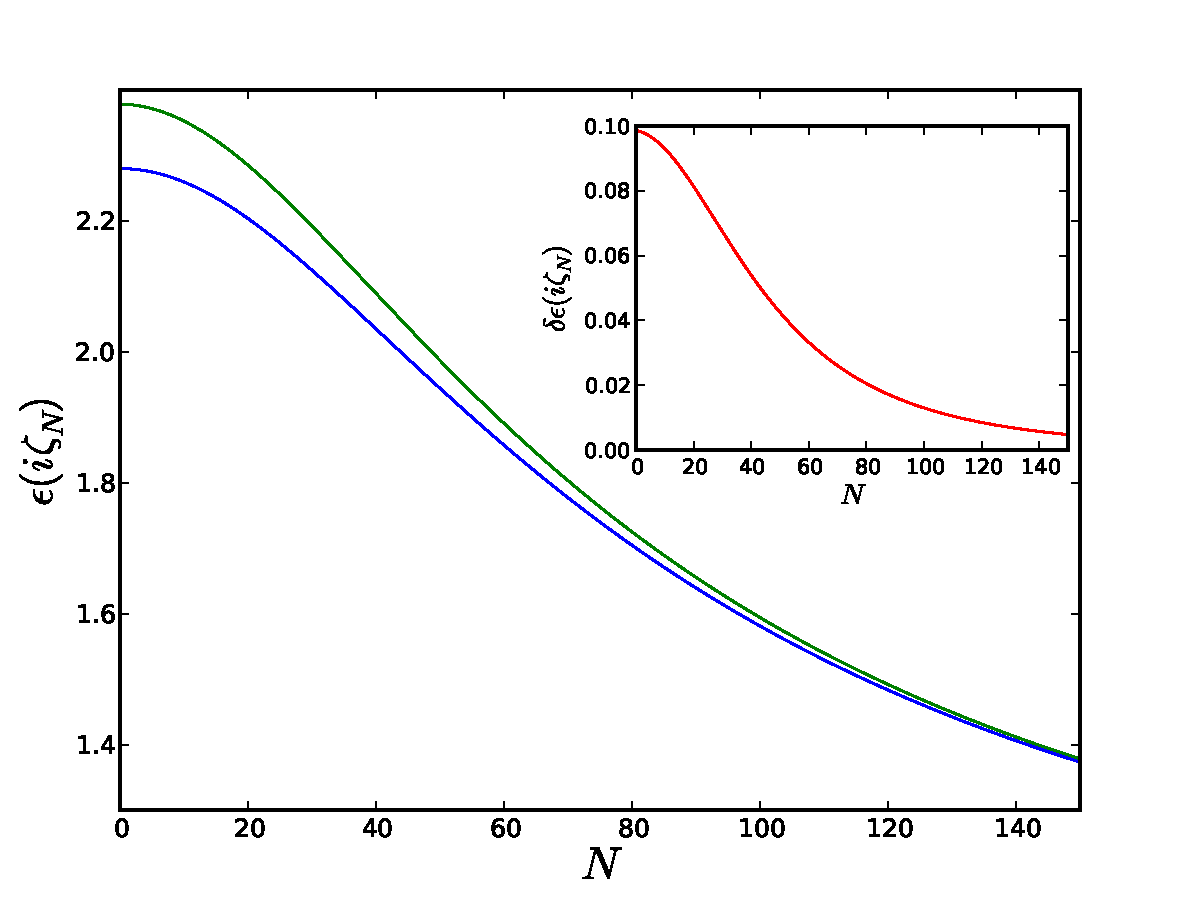
\includegraphics[width=1.2\textwidth]{./130807_plots/fig2b_eiz_deiz.pdf} (b)
\end{center}
\end{minipage}
\caption{(a) The dielectric dispersion spectrum $\epsilon''(\omega)$ as a  function of frequency $\omega$ in the units of $\rm [10^{16} ~s^{-1}]$ for amorphous silica without the exciton peak (blue line) and with a simulated exciton peak (green line). The inset shows the difference between the two spectra as a function of frequency. (b) The Kramers-Kronig transform $\epsilon(i \zeta_N)$ without (blue line) and with (green line) the exciton peak, as a function of the index $N$ of . The inset again shows the difference.}
\label{fiddle2}
\end{center}
\end{figure*} 

Fitting the calculated dependence of $Max\left(\delta{\cal A}(i\zeta)\right)$ on ${\cal C}$, it is possible to extract the following behavior for the frequency of this maximum, $\zeta_{max}$, as 
\begin{equation}
\zeta_{max} \sim \left\{
\begin{array}{cc}
0 &;  {\cal C} < {{\cal C}_0} \\
~ & ~ \\
 \omega_0 ~ \sqrt{{\cal C}-{{\cal C}_0}} &;  {\cal C} \geq {\cal C}_0, \\
\end{array}\right.  
\label{nkgslkj}
\end{equation}
%for $\omega_0   = \tilde\omega$,
%\begin{equation}
%\zeta_{max} = \left\{
%\begin{array}{cc}
%0 &;  {\cal A} < {{\cal A}_2} \\
%~ & ~ \\
%\sqrt{\omega_0} ~C''~  ({\cal A}-{{\cal A}_2})^{0.47}&;  {\cal A} \geq {\cal A}_2, \\
%\end{array}
%\right.  
%\end{equation}
where ${\cal C}_0 = 7.38$ can be read off Fig. \ref{fiddle1}(a), and ${\cal C} = \frac{\pi}{2}(\varepsilon(0) - 1).$ Obviously, spectra with larger static dielectric constants, specifically $(\varepsilon(0) - 1) > 4.7$, would lead to a maximum in the vdW interaction free energy variation at frequencies that scale linearly with $\omega_0$.  Furthermore, the numerical coefficient in Eq. \ref{nkgslkj} as well as ${\cal C}_0$ are both functions of the ratio ${\omega_0}/{\tilde\omega}$. The dependence of $\zeta_{max}({\cal C}, {\omega_0}/{\tilde\omega})$  is presented in Fig. \ref{fiddle1}(b). It is clear that ${\cal C}_0$ changes only marginally for ${\omega_0}/{\tilde\omega} > 2$ but has an important effect for ${\omega_0}/{\tilde\omega} < 1$. Apart from this, qualitatively, the functional form of $\zeta_{max}$ is very similar in the whole parameter space. It is indeed quite unexpected that the affect of addition of a lone peak to the dielectric spectrum would effect the different frequency terms in the Matsubara sum of the vdW interaction free energy in such a non-monotonic fashion. 

%There is not even a semblance of the many time assumed direct connection between the added peak characteristic frequency and the corresponding Matsubara sum behaviour.

The relation between the spectral change and the Matsubara frequency at which there is the largest change of the vdW interaction free energy is thus quite complicated and extremely indirect. It depends on overall properties of the complete dielectric spectrum as exemplified by ${\cal C}$ and ${\tilde\omega}$. Though these results can be derived explicitly only for the very simple toy model explained above, the salient features revealed remain true even in more realistic cases, as we will elucidate below. 


\subsection{Interaction free energy variation: realistic spectrum variation}

We now apply our general formulation of the dielectric response variation and the consequent interaction free energy variation to the case of an exciton peak in amorphous silica. This is aimed at elucidating the often posed, but never properly answered question,  what exactly is the effect of addition or removal of a single sharp (exciton) peak on the vdW interaction free energy.

For the non-perturbed dielectric dispersion spectrum, we take the imaginary part of the dielectric permittivity, $\epsilon''(\omega)$, of amorphous silica, as calculated with the OLCAO-DFT methodology by Ching et al. \cite{silica}. Being a one-electron approximation, the calculated spectrum does not contain any exciton effects; the corresponding peak measured by Tan et al. \cite{Tan} is missing.  In order to simulate an additional excitonic peak, we next synthesize a modified spectrum by adding a Lorentz oscillator peak just below the fundamental absorption edge of the OLCAO-DFT calculated dielectric dispersion spectrum, at a frequency $ \omega_0 = 1.245 \times 10^{16}~s^{-1}$. The magnitude, position, and full width at half maximum (FWHM) of this Lorentz oscillator peak were determined by comparison with experimental spectra \cite{Tan}, so that the ratios of both the position and magnitude of the exciton peak to the first interband transition peak were the same in the experimental spectrum and our synthesized spectrum. The FWHM of the added Lorentz oscillator peak is the same as that of the exciton peak in the measured spectrum. Finally, the whole synthesized spectrum was rescaled so that the total oscillator strength of the spectrum was unchanged by the addition of the Lorentz oscillator peak and that the number of electrons does not depend on the way the spectrum is constructed. It remains an invariant.

\begin{figure}[t!]
\begin{center}
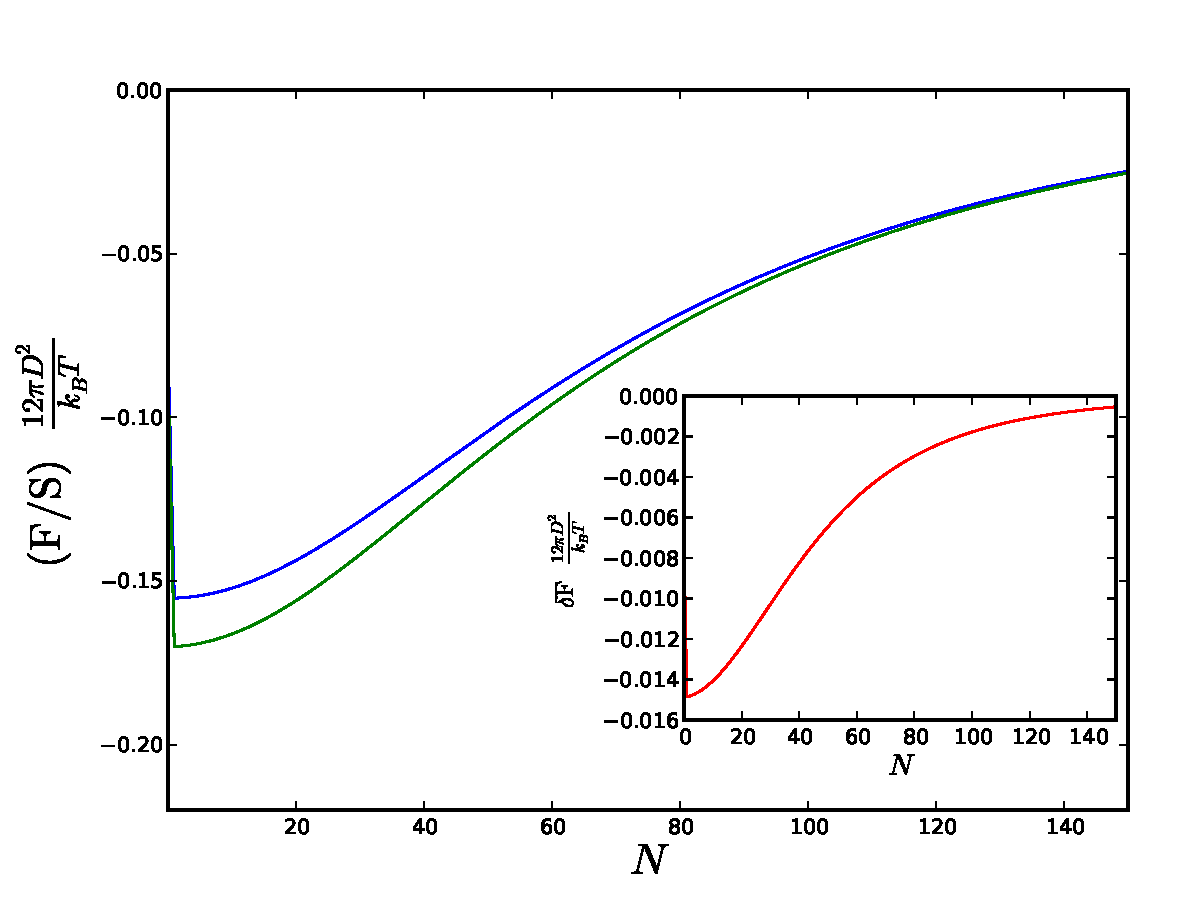
\includegraphics[width=0.5\textwidth]{./130807_plots/fig3_F_dF.pdf} 
\end{center}
\caption{The variation of the different Matsubara frequency components in the Hamaker coefficient summation (Eq. \ref{vdxahj}). The x-axis shows the index $N$ of the Matsubara frequencies $\zeta_N$. The biggest change is associated with the lowest frequency terms. The difference between the two curves is given almost exactly by the first order correction, Eq. \ref{ncirselunh}, and is shown in the inset as a function of the Matsubara frequency components.}
\label{fiddle3}
\end{figure} 

From Fig. \ref{fiddle2}(a) we discern that the addition of the Lorentz oscillator peak affects all or most of the imaginary part of the dielectric spectrum. The imposition of the oscillator sum rule has the most significant effect only in a narrow frequency interval centered around the fundamental absorption edge, showing a weak tail at larger frequencies.  Expectably the corresponding Kramers-Kronig transform of the dispersion spectrum $\epsilon(i \zeta)$ shown in Fig. \ref{fiddle2}(b) shows the largest  variation close to the static $\zeta = 0$ region but has a finite variation distributed throughout the whole range of imaginary frequencies. Obviously the non-local connection between $\epsilon'' (\omega)$ and $\epsilon(i \zeta)$, provided by the Kramers-Kronig transform, Eq. \ref{cgsrlhjk}, shows up in their quite distinct dependence on the addition of an extra Lorentz oscillator peak. 

The effect of peak addition on the corresponding terms in the Matsubara sum for the non-retarded Hamaker coefficient (Eq. \ref{vdxahj}) is shown in Fig. \ref{fiddle3}.  Clearly, the largest variation of about 10 \% is observed for lowest Matsubara terms, closest to the static limit. We are thus in the $\zeta_{max} = 0$ limit, see Fig. \ref{fiddle1}.  

After summing up the Matsubara terms, the total change of the Hamaker coefficient then amounts to $\delta {\cal H} = -5.03~ zJ$ and is proportional to the area between the two curves in Fig.  \ref{fiddle3}. The value of the Hamaker coefficient for the unperturbed spectrum is $84.9~ zJ$. The relative change in the Hamaker coefficient is thus $\sim 6$ \%. Considering that this change is due to the presence of a single narrow Lorentzian peak in the dielectric spectrum of the interacting material, it is non-negligeable. We note that the first-order (linear) correction to the interaction free energy (Eq. \ref{ncirselunh}) reproduces the change in the Hamaker coefficient almost exactly and thus points to the conclusion that addition of multiple peaks would simply contribute additively to the overall change of the Hamaker coefficient.

\begin{figure*}[t!]
\begin{center}
\begin{minipage}[b]{0.45\textwidth}
\begin{center}
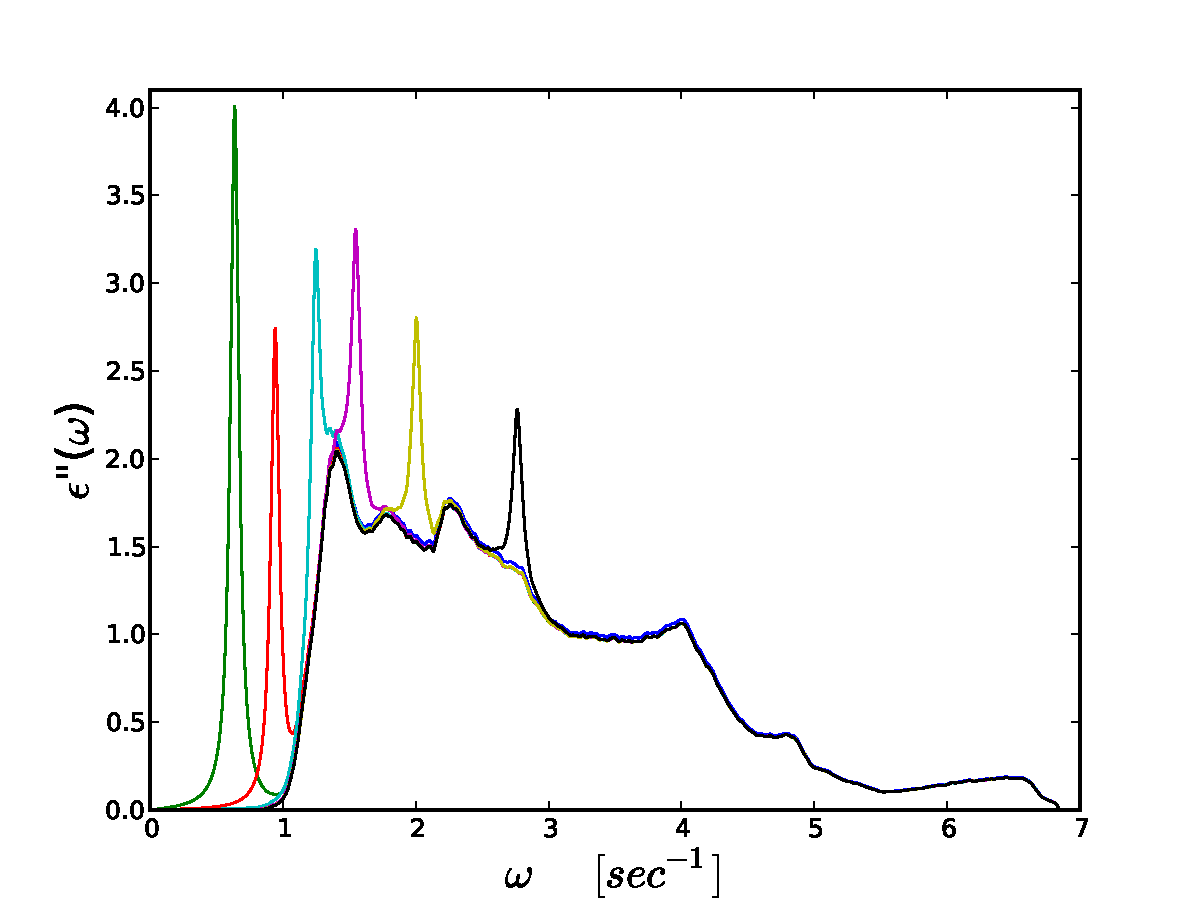
\includegraphics[width=1.2\textwidth]{./130807_plots/fig4a_shifted_peaks_eps2.pdf} (a)
\end{center}
\end{minipage}
\hskip 34pt
\begin{minipage}[b]{0.45\textwidth}
\begin{center}
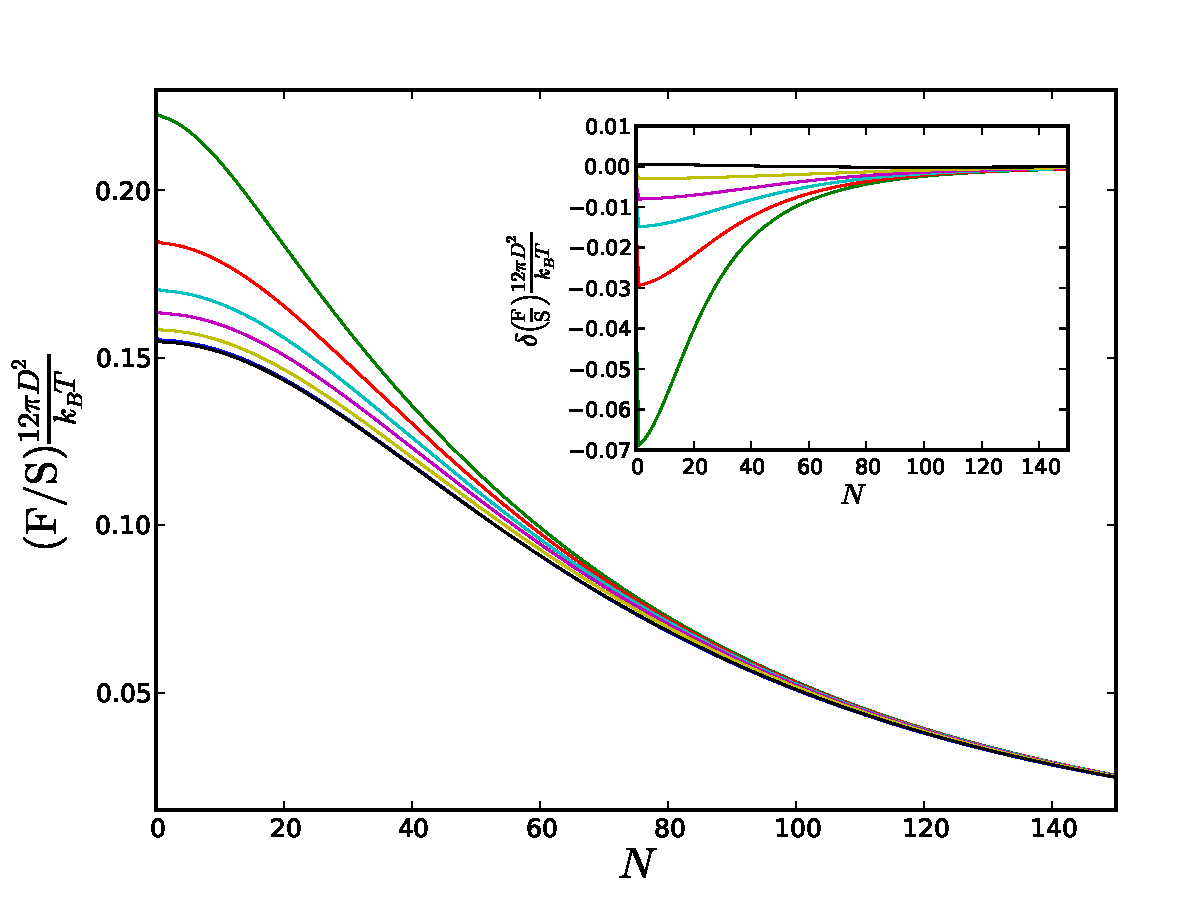
\includegraphics[width=1.2\textwidth]{./130807_plots/fig4b_shifted_peaks_F_dF.pdf} (b)
\end{center}
\end{minipage}
\caption{(a) The background dielectric dispersion spectrum $\epsilon(\omega)$ of amorphous silica without the exciton peak in the frequency interval $\rm 0 - 6.88 \times 10^{16}~s^{-1}$, (black line), and the synthesized spectrum with an added (exciton) Lorentzian peak at various frequencies in units of $\rm [10^{16} ~s^{-1}]$. (b) Terms in the interaction free energy summation, Eq. \ref{cfbr1}, as well as change in the Hamaker coefficient (inset), Eq. \ref{ncirselunh},  both as a function of the Matsubara frequency index. The biggest change is associated with the low frequency terms and peak position at lower frequencies.}
\label{fiddle4}
\end{center}
\end{figure*} 

We now modify the unperturbed calculated dielectric dispersion spectrum by adding a Lorentz oscillator peak at variable frequency positions, thus avoiding the constraint that the simulated excitonic peak should be just below the fundamental absorption edge. Again the FWHM and the oscillator strength of this added Lorentz oscillator peak were taken from with experimental spectra \cite{Tan}, while the position was chosen arbitrarily. The background spectrum was multiplied by a scaling factor so that that the oscillator strength at 43 eV ($\rm 6.88 \times 10^{16}~s^{-1}$) for the background spectrum with the additional Lorentzian peak matches the oscillator strength at 43 eV from the experimental spectrum as measured in Ref. \cite{Tan}. This guarantees that the effective number of electrons up to and including the energy 43 eV remains invariant. 

Fig. \ref{fiddle4}(a)  shows the imaginary part of the dielectric spectra for various peak positions as obtained from the forementioned rescaling. The dependence of the corresponding change in the Hamaker coefficient as a function of the Matsubara frequency is shown in Fig. \ref{fiddle4}(b). A broad range of behaviors is observed for the latter, but overall one notices that the peak position at lower frequency $\omega_0$ leads to larger changes in the Hamaker coefficient. This follows from the form of $\delta \varepsilon(i \zeta)$, Eq. \ref{ngkslh}, that depends on the ratio of ${\cal A}/\omega_0$.

Because of the rescalings implicit in the synthetic spectrum, in order to satisfy the sum rule up to the highest value of the frequency at which data are available for both spectra, the {\sl ab initio} and the experimental results, i.e., 43 eV or $\rm 6.88 \times 10^{16}~s^{-1}$, the frequency variation of the Matsubara terms in the Hamaker coefficient depends on the position of the peak. For peak positions at $\omega_0 = 0.638,  0,942,  1.245, 1.549, 2.005 ~{\rm and} ~2.764 \times 10^{16} ~s^{-1}$ the corresponding relative changes in the Hamaker coefficient amount to $\delta {\cal H}/{\cal H} = \rm -16.2 \%, -9.4 \%, -5.9 \%, -3.8 \%, -1.8 \% ~{\rm and} ~ 1 \%$. We can thus conclude that the simulation of spectra with an added peak confirm the insight of the toy model that the addition of peaks at smaller characteristic frequency $\omega_0$ and larger FWHM have a more pronounced effect on the Hamaker coefficient, and make it larger. In fact, one can deduce that the relative changes in the Hamaker coefficient are proportional to FWHM of the added peak and inversely proportional to its frequency $\omega_0$. 

\subsection{Discussion}

We investigated the quantitative relationship between the changes in the dielectric spectrum and the corresponding variation in the magnitude of the vdW interactions. Because the vdW interaction free energy is a functional of the Kramer-Kronig transform, itself a functional of the imaginary part of the dielectric function, the relationship between the characteristics of an added peak at a certain frequency and the Matsubara sum term for the Hamaker coefficient closest to that frequency is not direct. In fact, the Matsubara frequency at which the largest change to the Hamaker coefficient occurs varies non-linearly with the position of the added peak and its FWHM. The overall variation in the Hamaker coefficient is then proportional to the full width at half maximum of the added peak and inversely proportional to its frequency. Its total relative change spans values from a few and up to $\rm \sim 10$ \%, depending on the characteristics of the single added peak. In the case of more complicated variations of the dielectric response, corresponding to addition of several peaks, the total variation corresponds to the sum of variations for individual peaks and can be quite large.  

Some care is therefore necessary when estimating and/or predicting the expected changes in the vdW interactions wrought by changes in the dielectric spectrum. There is no linear correspondence between the interaction free energy variation and the spectral properties of the interacting media.

\subsection{Acknowledgments:}

This research was supported by the U.S. Department of Energy, Office of Basic Energy Sciences, Division of Materials Sciences and Engineering under Award DE-SC0008176 and DE- SC0008068.

\begin{thebibliography}{99}

\bibitem{Parsegian} V. A. Parsegian, \textsl{Van der Waals Forces} (Cambridge Press, 2005).

\bibitem{Bordag} M. Bordag, G. L. Klimchitskaya, U. Mohideen, and V. M. Mostepanenko,
{\em Advances in the Casimir Effect} (Oxford University Press, New York, 2009).

\bibitem{Isrealachvili} J. Israelachvili, {\sl Intermolecular and Surface Forces, Third Edition: Revised Third Edition}  (Academic Press; 3rd edition 2011).

\bibitem{Blaaderen} A. Van Blaaderen, R. Ruel and P. Wiltzius, %{\sl Template-directed colloidal crystallization}, 
Nature {\bf 385} 321 (1997).

\bibitem{Chaikin} See-Eng Phan et al., %{\sl Phase transition, equation of state, and limiting shear viscosities of hard sphere dispersions}, 
Phys. Rev. E {\bf 54} 6633 (1996).

\bibitem{Bonn} D. Bonn et al., %{\sl Direct Observation of Colloidal Aggregation by Critical Casimir Forces}, 
Phys. Rev. Letts. {\bf 103} 156101 (2009).

\bibitem{Shen} Y. Shen, H. Hoffmann, L. Jiang, J. Hao, Z. Liu, %{\sl Bilayer swelling of nonionic surfactant and sodium dodecylsulfate mixed system by refractive-index matching}, 
Colloid and Polymer Sci. {\bf 290} 1493 (2012).

\bibitem{Manohar} J. Narayanan and C. Manohar, %{\sl Helix – Rod transition in a nanospring}, 
J. of Coll. and Interf. Sci. {\bf 350} 200 (2010).

\bibitem{CNTexciton} M. S. Dresselhaus, G. Dresselhaus, R. Saito, and A. Jorio, Annu. Rev. Phys. Chem. {\bf 58} 719 (2007).

\bibitem{Measurable} M. S. Dresselhaus, G. Dresselhaus, R. Saito and A. Jorio, Phys. Rep.  {\bf 409} 47 (2005). M.S.Dresselhaus and P.C. Eklund, Adv.Phys. {\bf 49} 705 (2000).

\bibitem{Hobbie} E. K. Hobbie, T. Ihle, J. M. Harris, and M. R. Semler, Phys. Rev. B {\bf 85}, 245439 (2012).

\bibitem{DFT} W.-Y. Ching and P. Rulis, {\sl Electronic Structure methods for Complex Materials, The Orthogonalized Linear Combination of Atomic Orbitals}  (Cambridge University Press, Oxford University Press, 1st edn, 2012).

\bibitem{silica} Neng Li, Wai-Yim Ching, Journal of Non-Crystalline Solids, in press (2013).

\bibitem{Tan} G. L. Tan, M. F. Lemon, D. J. Jones, and R. H. French, Phys. Rev. B {\bf 72} 205117 (2005).

\bibitem{LLSPpart2} L. P. Pitaevskii and E.M. Lifshitz, {\sl Statistical Physics, Part 2: Volume 9 (Course of Theoretical Physics Vol. 9)} (Butterworth-Heinemann, 1980).

\bibitem{Abramowitz} M. Abramowitz and I. Stegun, {\sl Handbook of Mathematical Functions} (Dover New York, 1972).

\bibitem{Smith} D.Y. Smith, {\em Dispersion theory, sum rules and their application to the analysis of optical data}, in {\sl Handbook of Optical Constants of Solids},  E.D. Palik Ed. Academic Press, (1985) p.35.

\end{thebibliography}

%\bibitem{NinPar-water} B. Ninham and V.A. Parsegian, Biophys. J. {\bf 10} 646 (1970).

\end{document}
